\subsection{Docker jExam Infrastructur}
Um eine stabile Testinfrastruktur zu schaffen und eine bessere
Verwaltung der Container zu ermöglichen, wurde Docker-Compose
verwendet, um die verschiedenen Testdienste von jExam zu trennen
und zu gruppieren. So kann der Tester nur die Dienste ausführen,
die er braucht und die er testen will. Wenn alle Container
gleichzeitig gestartet würden, könnte dies sehr viele Ressourcen auf
dem Host-Computer beanspruchen und das gesamte System verlangsamen.
Da einige Dienste voneinander abhängig sind, wurde ein Docker-Netzwerk
geschaffen, das die Kommunikation zwischen den ausgeführten Diensten
ermöglicht. Dies ermöglicht ein geschlossenes lokales Netzwerk, das
von außen nicht einsehbar ist (siehe \Cref{fig:dock-net}).

\begin{figure}[H]
    \centering
    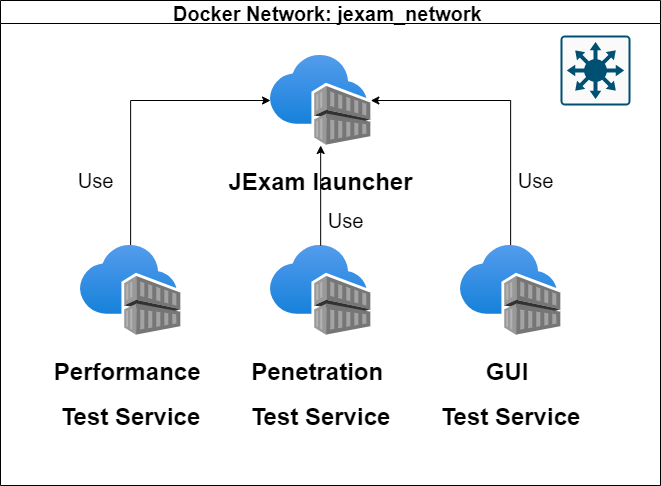
\includegraphics[scale=0.6]{images/all.drawio}
    \caption{jExam Docker Network Darstellung} \label{fig:dock-net}
\end{figure}

\subsubsection{jExam Launcher}

jExam Launcher ist der Hauptdienst der Docker Infrastruktur. Er ist für die Ausführung
und Bereitstellung von \gls{jexam_new} und \gls{jexam_2009} zuständig. Der Dienst
besteht aus fünf Containern, darunter :

\begin{itemize}
    \setlength\itemsep{1em}

    \item[] \textbf{JBoss}: Dieser Container enthält das Skript zum
    Bereitstellen des JBoss-Servers, den \gls{jexam_new} und \gls{jexam_2009}
    benötigen, um funktionieren zu können. Dieser Server dient auch
    als Datenbank für die beiden Apps. Er legt daher einige seiner
    Ports offen, um für externe Verbindungen zugänglich und offen
    zu sein.

    \item[] \textbf{Initializer}: Dieser Container enthält ein
    Java Skript, das automatisch (oder auf Wunsch des Testers auch
    manuell) ausgeführt wird und dazu dient, Testdaten in den 
    JBoss-Server zu injizieren. Es initialisiert die Daten, die für
    die Ausführung der Tests erforderlich sind.

    \item[] \textbf{OldWeb}: Dieser Container ermöglicht das
    Deployment von \gls{jexam_2009}. Er enthält einen Tomcat-Webserver,
    der den Code von \gls{jexam_2009} ausführt und sich dann mit
    dem Container verbindet, der den JBoss-Server enthält.
    Dieser Container legt ebenfalls seine Ports offen, damit er
    von den Tests erreicht werden kann, wenn diese im lokalen 
    Modus ausgeführt werden.

    \item[] \textbf{Webservice und Web}: Diese beiden Container
    ermöglichen die Ausführung und Bereitstellung von
    \gls{jexam_new}. Der Webservice enthält eine API, die vor
    allem mit dem JBoss-Server kommuniziert. Der Web-Container
    enthält das Frontend der Anwendung. Web verbindet sich mit
    dem Webservice, wenn er gestartet wird, und stellt Ports zur
    Verfügung, die ihn zugänglich machen, wenn die Tests im
    lokalen Modus gestartet werden.
\end{itemize}

\begin{figure}[H]
    \centering
    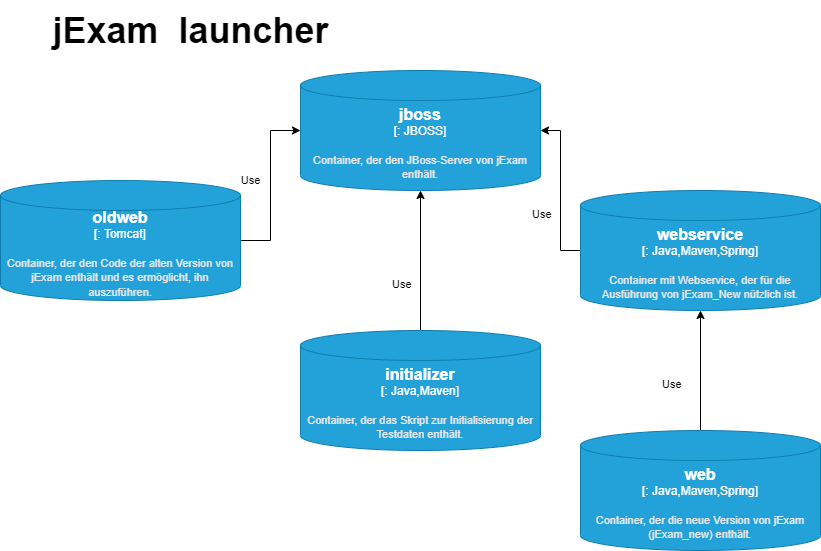
\includegraphics[scale=0.5]{images/launcher.drawio}
    \caption{jExam Launcher Testservice} \label{fig:laucher}
\end{figure}
\subsubsection{UI-Testservice}

Das UI-Testservice ist die Dienststelle, die für die Durchführung
von UI-Tests verantwortlich ist. Es besteht im Wesentlichen aus
vier Containern:

\begin{itemize}
    \setlength\itemsep{1em}

    \item[] \textbf{Selenium-Hub, Chrome- und Firefox-RemoteWebDriver}:
    Der Selenium Hub ist ein Server, der die Zugriffsanfragen vom 
    WebDriver-Client entgegennimmt und die JSON-Testbefehle an die 
    entfernten (remote) Driver weiterleitet. Er nimmt die Befehle vom 
    Client entgegen und führt sie parallel auf den verschiedenen 
    remote Driver aus. Dies ermöglicht die Verwendung der 
    RemoteWebDriver Chrome und Firefox, die direkt mit dem
    Selenium-Hub verbunden sind. Der Tester kann also wählen,
    welchen Browser er für die Ausführung seiner Tests verwenden
    möchte. Es ist jedoch wichtig, darauf hinzuweisen, dass die 
    Container, die die RemoteWebDriver enthalten, so konfiguriert 
    sind, dass sie mit der neuesten Version des Browsers ausgeführt 
    werden, die bei jedem Docker Image Build automatisch 
    heruntergeladen wird.

    \item[] \textbf{UI-Test}: Dieser Container enthält die UI-Tests
    und ist dafür zuständig, diese automatisch mithilfe eines
    Maven-Skripts auszuführen. Wenn die Tests im Remote-Modus
    konfiguriert sind, verbindet sich der Container mit dem
    Selenium-Hub, um Zugriff auf den verfügbaren RemoteWebDriver
    zu erhalten.
\end{itemize}

\begin{figure}[H]
    \centering
    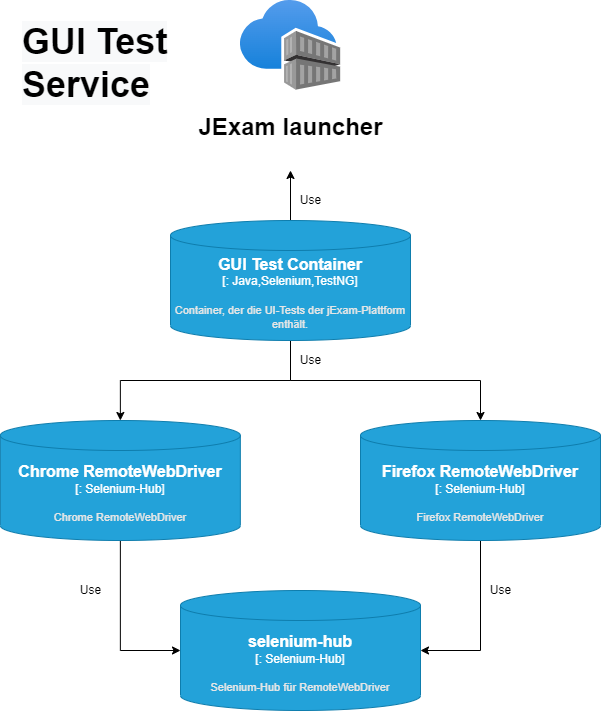
\includegraphics[scale=0.6]{images/gui.drawio}
    \caption{JExam UI Testservice} \label{fig:ui}
\end{figure}
\subsubsection{Penetration Testservice}

Das Penetration Testservice ist der Dienst, der für die Ausführung
von Penetrations- und Sicherheitstestskripten verantwortlich ist.
Dieser Dienst besteht aus einem einzigen Container:

\begin{itemize}
    \setlength\itemsep{1em}

    \item[] \textbf{Owasp}: Dieser Container besteht aus einem
    stabilen Abbild von Zapproxy und enthält die verschiedenen
    Skripte, die auf \Gls{jexam_new} und \Gls{jexam_2009}
    ausgeführt werden: zap-baseline und zap-fullscan.

\end{itemize}

\begin{figure}[H]
    \centering
    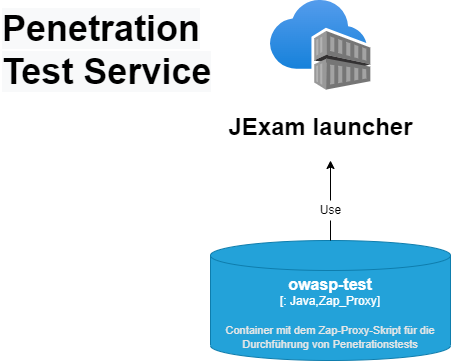
\includegraphics[scale=0.6]{images/penetration.drawio}
    \caption{JExam Penetration Testservice} \label{fig:pen}
\end{figure}

